\documentclass[11pt,letterpaper]{exam}
\usepackage[utf8]{inputenc}
%\usepackage[spanish]{babel}
\usepackage{graphicx}
\usepackage{float}
%\decimalpoint

\begin{document}
\begin{center}
{\Large Métodos Computacionales} \\
S4C1 tarea - \textsc{Makefile}\\
03-2023\\
\end{center}


\noindent
\section{Gr\'aficas}
\begin{center}
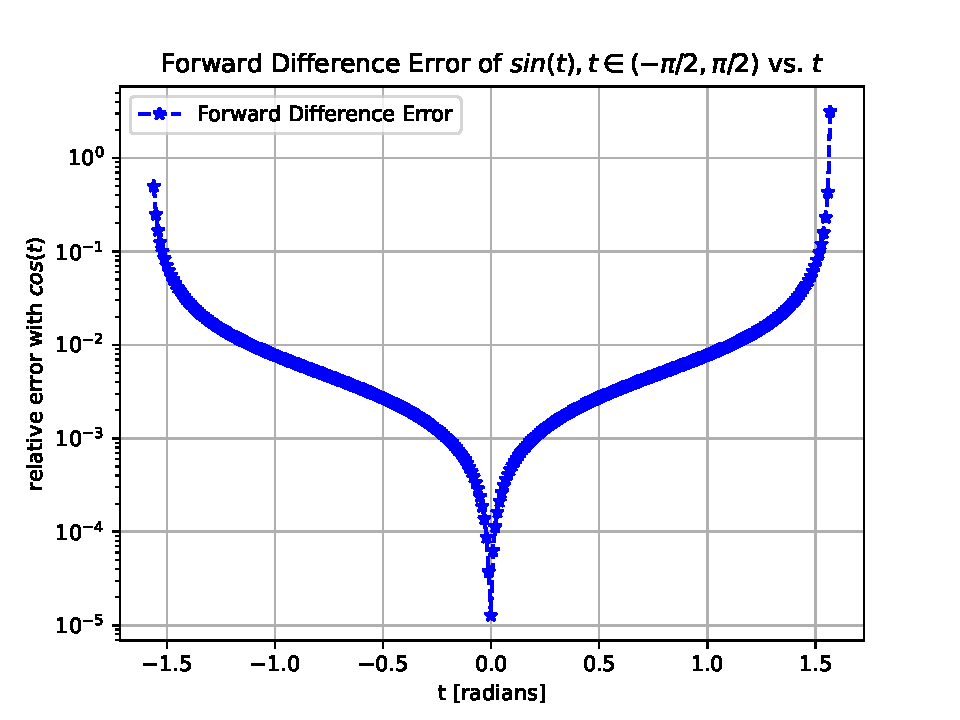
\includegraphics[width=10cm]{err_derF.pdf}
En los extremos el error es mayor que para los valores del centro.
\begin{center}
\end{center}
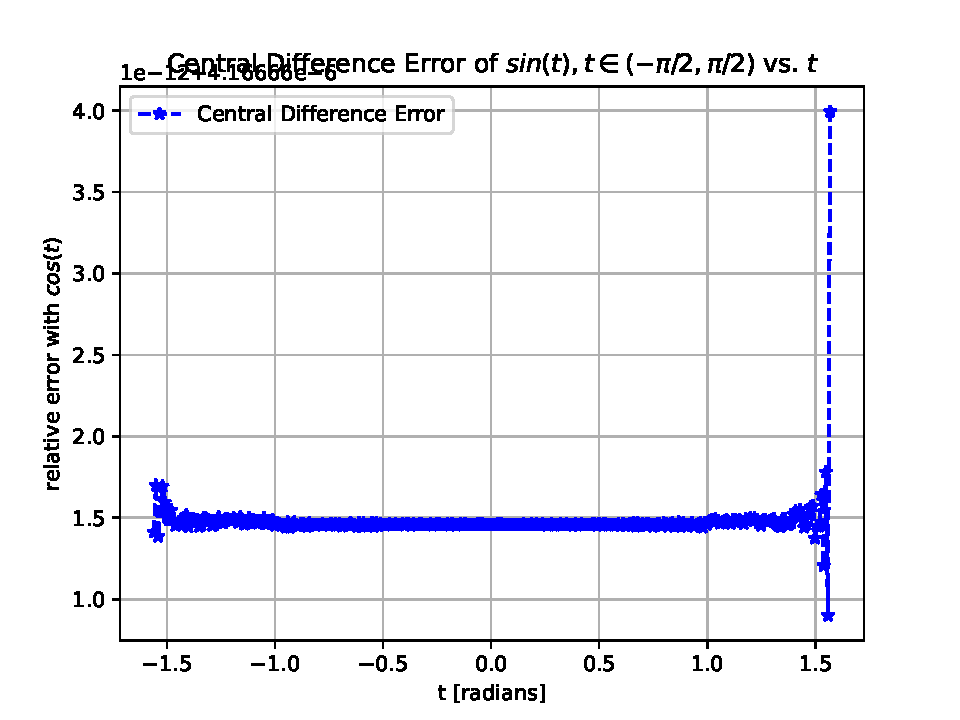
\includegraphics[width=10cm]{err_derC.pdf}
El error en este método se mantiene en la misma magnitud todo el tiempo, al rededor de $10^{-6}$.  
\end{center}
\begin{center}
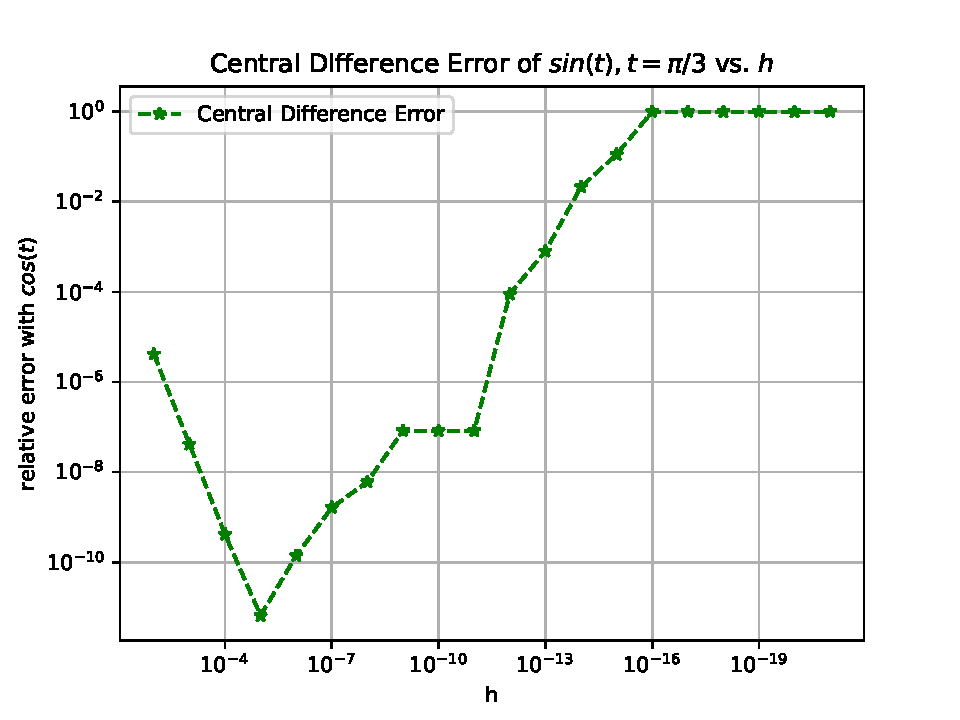
\includegraphics[width=10cm]{err_der_h.pdf}
El error disminue hasta ciero $h$ para luego incrementarse por el error computacional acumulado. 
Obsérvese que el error tiene una magnitud de $10^{-6}$ cuando $h=0.01$ coincidiendo con la gráfica anterior.
\end{center}
\end{document}
